\documentclass[a4paper, 12pt, final, garamond]{book}
\usepackage{cours-preambule}
\graphicspath{{./figures/}}

\raggedbottom

\makeatletter
\renewcommand{\@chapapp}{Programme de kh\^olle -- semaine}
\makeatother

\begin{document}
\setcounter{chapter}{12}

\chapter{Du 06 au 9 janvier}

\section{Cours et exercices}
\subsection(E8){Filtrage linéaire}
\begin{enumerate}[label=\Roman*]
	\item[b]{Décomposition en série de Fourier}~: théorème de
	      \textsc{Fourier}, analyse spectrale, relation de \textsc{Parseval}.
	\item[b]{Filtrage linéaire}~: introduction, notion de filtre et de fonction de
	      transfert, exemple filtre RC sur C~; effet d'un filtre sur un signal
	      périodique composé.
	\item[b]{Description d'un filtre}~: gain et gain en décibel, échelle
	      logarithmique~; lien entre amplitude et gain en décibel, application RC
	      sur C~; diagramme de Bode, définition et exemple, diagramme asymptotique
	      et application RC sur C~; lecture d'un diagramme de Bode~; types de
	      filtres (moyenneur, intégrateur, dérivateur).
	\item[b]{Exemples de filtres}~: RC sur C, passe-bas, intégrateur, RC sur R,
	      passe-haut, dérivateur, RLC sur C, passe-bas ordre 2, RLC sur R,
	      passe-bande~; filtres en cascade et résumé.
\end{enumerate}

\subsection(ON1){Ondes progressives}
\begin{enumerate}[label=\Roman*]
	\item[b]{Introduction}~: signal, perturbation, onde, propagation.
	\item[b]{Onde progressive à une dimension}~: définition, représentation
	      spatiale, célérité, représentation temporelle, retard, lien entre les
	      représentations.
	\item[b]{Onde progressive sinusoïdale}~: définition, double
	      périodicité et rappel spectre électromagnétique, expression mathématique
	      de l'OPS, vitesse de phase.
	\item[b]{Milieux dispersifs}~: définition, exemples.
\end{enumerate}

\section{Cours uniquement}
\subsection(ON2){Interférences à deux ondes}
\begin{enumerate}[label=\Roman*]
	\item[b]{Introduction}~: approximation par une onde plane, phase spatiale et
	      déphasage, rappel valeurs particulières, différence de marche et
	      correspondance valeurs particulières pour $\Delta{\f_0} = 0$.
	\item[b]{Superposition d'ondes sinusoïdales de mêmes fréquences}~:
	      préesntation, signaux de même amplitude, signaux d'amplitudes différentes,
	      bilan, exercice d'application.
	\item[b]{Interférences lumineuses}~: cohérence, intensité, formule de
	      \textsc{Fresnel}, chemin optique.
	\item[b]{Expérience des trous d'\textsc{Young}}~: introduction,
	      présentation, détermination de l'interfrange.
\end{enumerate}

\newpage

\section{Questions de cours possibles}
\subsection(E8){Filtrage linéaire}
\begin{enumerate}
	\item Pour un des filtres ci-dessous~: présenter le système réel, le système
	      en RSF, déterminer sa fonction de transfert, son gain en décibels, son
	      déphasage, déterminer les asymptotes et tracer les diagrammes de
	      \textsc{Bode}.
	      \begin{tasks}[label=\protect\fbox{\Alph*}](4)
		      \task RC sur C (E8|IV/A)
		      \task RC sur R (E8|IV/B)
		      \task RLC sur C (E8|IV/C)
		      \task RLC sur R (E8|IV/D)
	      \end{tasks}
	\item Définir les trois effets de filtres étudiés~: moyenneur, intégrateur
	      dérivateur (Df.E8.7). Donner les formes canoniques des filtres passe-bas et
	      passe-haut d'ordre 1 (Ipt.E8.1 et 2) et démontrer leur comportement
	      intégrateur ou dérivateur (Pt.E8.3 et 4). Représentez l'effet d'un
	      intégrateur sur un signal créneau et l'effet d'un intégrateur sur un signal
	      triangle (Ex.E8.4 et 5).
	      \subsection(ON1){Ondes progressives}
	\item Démontrer le lien entre les représentations spatiales et temporelles
	      pour une ondes progressive à 1 dimension se propageant dans le sens des $x$
	      croissants à la célérité $c$ constante (Dm.ON1.1). Que se passe-t-il si l'on
	      va dans le sens des $x$ décroissants~? (At.ON1.1)
	\item On considère ici une vague solitaire qui se déplace à la vitesse $c =
		      \SI{18}{km.h^{-1}}$ le long d'un fleuve rectiligne, et on définit un
	      axe $(Ox)$ dans la direction du sens de sa propagation. À l'instant
	      $t=0$, le profil du niveau de l'eau du fleuve a l'allure suivante~:
	      \begin{center}
		      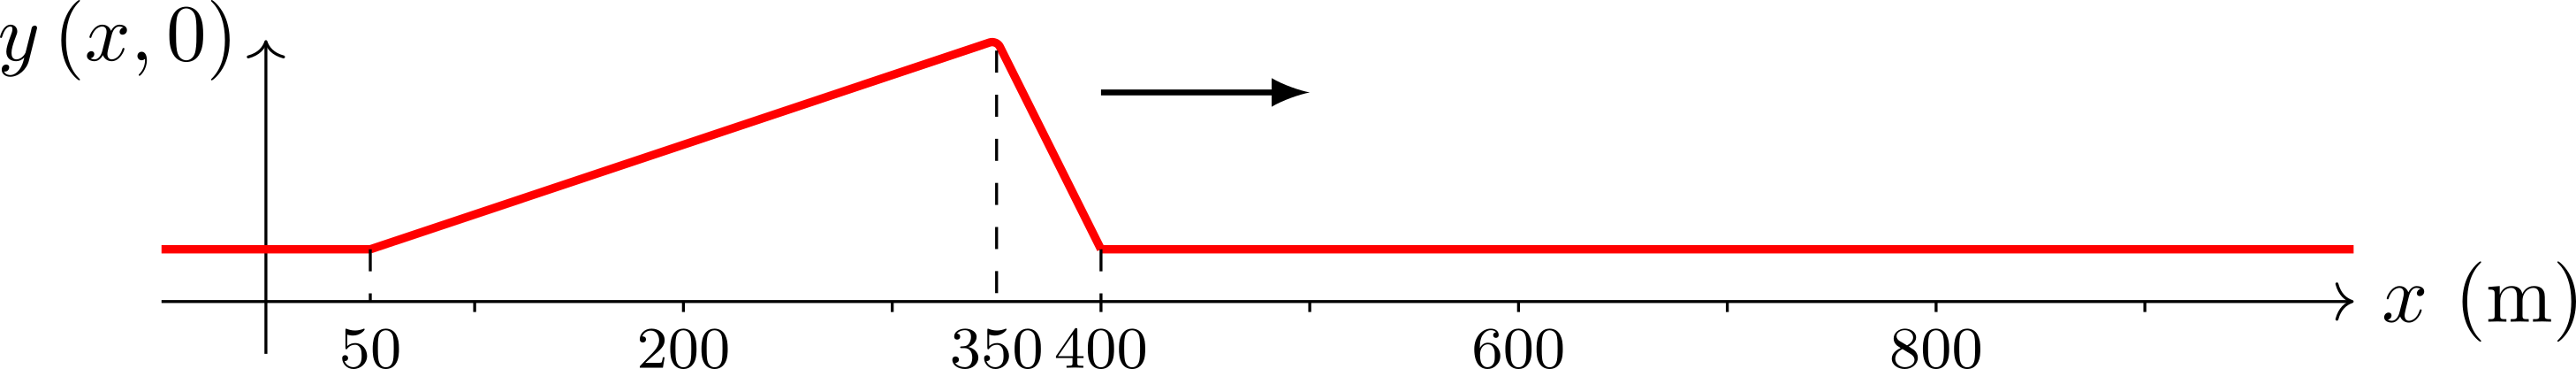
\includegraphics[width=0.8\linewidth]{rep_spa-masc_a}
	      \end{center}
	      \begin{enumerate}[label=\sqenumi]
		      \item Faire un schéma du profil du fleuve à $\tau = \SI{1}{min}$ en
		            supposant que l'onde se propage sans déformation.
		      \item Un détecteur fixe, enregistrant la hauteur du fleuve en fonction
		            du temps, est placé à l'abscisse $x_d = \SI{1.6}{km}$. Dessiner
		            l'allure des variations $y(x_d,t)$ en fonction du temps à cette
		            abscisse.
	      \end{enumerate}
	\item Présenter ce qu'est une onde progressive sinusoïdale (Df.ON1.6).
	      Démontrer alors l'expression générale d'une OPS (Dm.ON1.1). Indiquer les
	      différentes relations reliant~:
	      \begin{tasks}[label=\protect\fbox{\Alph*}](3)
		      \task $\omega$ et $f$ ou $T$~;
		      \task $\lambda$, $c$ et $f$ ou $T$ (Ipt.ON1.4).
		      \task $k$ et $\lambda$ (Df.ON1.8)~;
	      \end{tasks}
	      % \item Répondre à au moins 2 questions parmi les suivantes (nombre au
	      % choix de
	      % l'interrogataire)~:
	      % \begin{enumerate}
	      % \item Soit $f(t)$ la fonction modélisant un signal en $x=0$. Donner et
	      % démontrer l'expression du signal $s(x,t)$ en M$(x)$ ($x>0$) en
	      % considérant une onde qui se propage vers les $x$ croissants de O à M
	      % à la célérité $c$ en fonction de $f$.
	      %
	      % \item Soit $f(t)$ la fonction modélisant un signal en $x=0$. Donner
	      % et démontrer l'expression du signal $s (x,t)$ en M$(x)$ ($x<0$) en
	      % considérant une onde qui se propage vers les $x$ décroissants de O
	      % à M à la célérité $c$ en fonction de $f$.
	      %
	      % \item Soit $g(x)$ la fonction modélisant un signal en $t=0$. Donner
	      % et démontrer l'expression du signal $s (x,t)$ en M$(x)$ ($x<0$) en
	      % considérant une onde se propageant vers les $x$ décroissants à la
	      % célérité $c$ en fonction de $g$.
	      %
	      % \item Une onde progressive sinusoïdale d'amplitude $A_0$ et de
	      % longueur d'onde $\lambda$ se propage dans le sens des $x$
	      % décroissants à la célérité $c$. La phase à $t=0$ au point A
	      % d'abscisse $x_A = {\lambda}/{4}$ est nulle. Donner l'expression
	      % de la fonction $s(x,t)$ en fonction de $A_0$, $\lambda$, $c$,
	      % $x$ et $t$. Quel est le déphasage entre A et l'origine O du
	      % repère~?
	      %
	      % \item Une onde sinusoïdale se propage dans la direction de l'axe
	      % $(Ox)$ dans le sens négatif avec la célérité $c$. On donne~:
	      % \hfill
	      % $\boxed{s_2(0,t) = A \sin(\omega t)}$
	      % \hfill~
	      % \smallbreak
	      % Déterminer l'expression de $s_2(x,t)$. Représenter graphiquement
	      % $s_2(\lambda/4,t)$ et $s_2(\lambda/2,t)$ en fonction de $t$.
	      % \end{enumerate}
	      \subsection(ON2){Interférences à deux ondes}
	\item Démontrer le lien entre déphasage et différence de marche (Df.ON2.2,
	      Pt.ON2.2, Dm.ON2.1). Démontrer les valeurs particulières de différence de
	      marche en précisant la condition pour les exprimer ainsi (Dm.ON2.2). Définir
	      et démontrer le chemin optique d'un rayon lumineux, et donner le lien entre
	      entre déphasage et chemin optique (Df.ON2.5, Dm.ON.9, Pt.ON2.11).
	\item Déterminer l'expression du signal somme de deux ondes sinusoïdales de
	      même fréquence \textbf{et même amplitude} (Pt.ON2.4, Dm.ON2.3). On
	      rappelle la formule de trigonométrie
	      \[
		      \cos p + \cos q =
		      2\cos(\frac{p-q}{2}) \cos(\frac{p+q}{2})
	      \]
	      Détailler les cas extrêmes et les valeurs de déphasage correspondantes
	      (Pt.ON2.5, Dm.ON2.4). Qu'est-ce qui change si les signaux n'ont pas la
	      même amplitude (Ipt.ON2.2)~? Définir les termes d'interférences
	      constructives et destructives. (Ipt.ON2.3)
	\item[s]"3" %
	      Déterminer l'expression du signal somme de deux ondes sinusoïdales
	      d'\textbf{amplitudes différentes} (Pt.ON2.6, Dm.ON2.5). Étude des cas
	      extrêmes (Pt.ON2.7, Dm.ON2.6) si le temps le permet.
	      \smallbreak
	      On donnera les expressions trigonométriques demandées par l'étudiant-e.
	\item{}(Ap.ON2.1)%
	      Soient 2 émetteurs envoyant une onde progressive sinusoïdale de même
	      fréquence, amplitude et phase à l'origine. Le premier est fixé à
	      l'origine du repère, l'émetteur 2 est mobile et à une distance $d$ du
	      premier, et un microphone est placé à une distance fixe $x_0$ de
	      l'émetteur 1 et est aligné avec les deux émetteurs. On néglige
	      l'influence de l'émetteur 2 sur l'émetteur 1 et toute atténuation.
	      \begin{enumerate}[label=\sqenumi]
		      \item \textbf{Faire un schéma}.
		      \item On part de $d=0$ et on augmente $d$ jusqu'à ce que le signal
		            enregistré soit nul. Ceci se produit pour $d_1 =
			            \SI{6.0}{cm}$. \textbf{Expliquer cette extinction} et en
		            déduire la longueur d'onde du signal.
		      \item Pour $d_2 = \SI{12.0}{cm}$, quelle sera
		            l'amplitude du signal enregistré~?
	      \end{enumerate}
	\item Expliquer ce qu'est la cohérence (Df.ON2.4) et pourquoi on ne fait des
	      interférence qu'avec une unique source pour des signaux lumineux (Pt.ON2.8).
	      Donner et justifier/démontrer l'expression de l'intensité d'un signal en
	      général et pour une OPS (Pt.ON2.9, Dm.ON2.7). Démontrer la formule de
	      \textsc{Fresnel} pour deux signaux sinusoïdaux de même fréquence et
	      d'amplitudes différentes. La simplifier pour des signaux de même
	      amplitude (Pt.ON2.10, Dm.ON2.8).
	\item Trous d'\textsc{Young}~: présenter l'expérience (Df.ON2.7) et démontrer
	      l'expression de l'intensité relevée dans le cas de signaux de même
	      intensité. En déduire l'expression de l'interfrange (Pt.ON2.12,
	      Dm.ON2.10).
	      \smallbreak
	      On donne le développement limité suivant~:
	      \[\sqrt{1+\ep} \ste(un){=}{\ep \ll 1} 1 + \ep/2 + o(\ep)\]
\end{enumerate}

\end{document}
